\documentclass[a4paper]{scrreprt}
\usepackage[german]{babel}
\usepackage[utf8]{inputenc}
\usepackage{graphicx}
\usepackage{pdflscape}

\begin{document}
\title{Implementierungsdokument}
\author{Hanselmann, Hecht, Klein, Schnell, Stapelbroek, Wohnig}
\maketitle 
\tableofcontents	
\listoffigures


\chapter{Einleitung}
Dieses Dokument beschreibt die Implementierungsphase einer Praxis der Softwareentwicklungsgruppe am Karlsruher Institut für Technologie. Der Titel der Gruppenaufgabe lautet: \textit{Entwicklung eines Werkzeugs zur Analyse formaler Eigenschaften von Wahlverfahren}. \\
Diese Dokument stellt die in dieser Phase entstandenen Unterschiede zu den vorherigen Phasen (Pflichtenheft und Entwurf) dar und erklärt, warum diese notwendig wurden. \\
Weiterhin wird die zeitliche sowie die personelle Aufteilung der Implementierung vorgestellt. \\
\section{Ziel des Programmes}
Ziel des Programmes ist es eine Lösung zur Analyse von formalen Eigenschaften von Wahlverfahren zu präsentieren. Zur Analyse der Eigenschaften wird Bounded Model Checking (Glossareintrag) verwendet. Der verwendete Bounded Model Checker ist CBMC (Glossareintrag). Das Programm soll folgende Module  bereitstellen: 
\begin{itemize}
\item Eine Möglichkeit zur Beschreibung eines Wahlverfahrens in der Programmiersprache C. 
\item Eine Möglichkeit zur Beschreibung von Eigenschaften, auf die das Wahlverfahren geprüft werden soll. Die Beschreibung erfolgt in einer Makrosprache (Glossareintrag).
\item Eine Möglichkeit zum Angeben der Parameter für welche das angegebenen Wahlverfahren analysiert werden soll (Anzahl Wähler, Anzahl Kandidaten, Anzahl Sitze). 
\item Eine Möglichkeit, die Analyse auszuführen.
\item Eine Ausgabe des Ergebnisses der Analyse: Eine Erfolgsmeldung falls alle Eigenschaften erfüllt werden und Präsentation eines Gegenbeispiels sonst.
\end{itemize}


\chapter{Unterschiede zu den im Pflichtenheft gestellten Kriterien}

\section{Musskriterien}
Falls Ein Kriterium nicht implementiert wurde, ausführlich begründen warum nicht.

\section{Sollkritierien}
\section{Kannkriterien}

\subsection{/FK1130/- Code Completion C-Editor}
Das automatische Schließen von Klammern und Anführungszeichen ist implementiert. Vorschlagen von Wörtern ist weder primitiv noch intelligent implementiert, da dies zeitlich noch mindestens 8 Mannstunden in Anspruch nehmen würde, und wir diese Zeit nicht haben.

\subsection{/FK1140/- Durch den User konfigurierbares Verhalten C-Editor}
Die Interfaces um diese Anforderungen zu implementieren existieren zwar, es fehlt allerdings an der Zeit dies jetzt noch fertig zu stellen (6-8 Mannstunden).

\subsection{/FK2140/ - Code Completion Eigenschafteneditor}
Fehlt vollständig da die Zeit von mindestens 8 Mannstunden fehlt.

\chapter{Änderungen am Entwurf}
Bspw. \\
Änderung abstrakte Fabrik in highlevel ist jetzt keine Abstrakte Fabrik mehr.\\ Dieses Entwurfsmuster konnte nicht verwendet werden, da die zu erstellenden Objekte teilweise voneinander abhängig sind. Weiterhin gibt es Objekte, die mehrere Rollen einnehmen, d.h. sie implementieren unterschiedliche Interfaces. \\
Die Lösung des Problems bietet ein so von uns genannter CentralObjectProvider der, bei seiner eigenen Konstruktion alle anderen Highlevelobjekte baut und diese dann über get zu Verfügung stellt.
Somit hat der BEASTCommunicator immer noch eine abstrakte Sicht auf alle Interfaces.

\section{CodeGenerierung}

Die Klasse CBMCCodeGeneration ist nicht mehr statisch. \\
Sie wird in der Implementierung von der Klasse CBMCProcessFactory instantiiert. \\
So wird für jedes erzeugte C-Tempfile (Glossareintrag) eine neue Instanz erstellt. Sinnvoll, da es es genau von den Parametern abhängt. \\
Jede Instanz der Klasse CBMCCodeGeneration erstellt eine Instanz eines CBMCCodeGenerationVisitor. \\
Dieser besitzt 2 neue Methode, die einstellen ob er zur Codegenerierung einer Vor- oder Nachbedingungen eines Wahlverfahrens verwendet wird.  \\
(Verändertes Klassendiagramm hier)

\section{UserActions}
Alle \verb!UserActions! der vier GUIs haben jetzt nur noch einen Verweis auf den ihnen zugehörigen Controller, und holen sich von diesem mit Gettern die von ihnen gebrauchten Klassen (FileChooser, SaveBeforeChangeHandler..). Beispielhaft am \verb!BooleanExpEditor! gezeigt:
\newline

(Diagramm folgt)
\newline

\section{SaverLoader}
PostAndPrePropertiesDescriptionSaverLoader, ElectionDescriptionSaverLoader, ParameterCheckParameterSaverLoader und ProjectSaverLoader implementieren nun das Interface SaverLoader mit den dargestellten Methoden. Dies ermöglicht es der Klasse FileChooser, polymorph gegebene DatenTypen abzuspeichern und gegebene Dateien zu laden.
Alle anderen \verb!SaverLoader!-Klassen haben nur statische Methoden.
Zudem gibt es noch eine \verb!StringSaverLoader! Klasse die mit \verb!createSaveString! aus allen vom Nutzer editierbaren Strings alle Vorkommen von ">" durch ">>" ersetzt, bzw. dies mit !\verb!createFromSaveString! rückgängig macht. Dies verhindert die Erstellung von nicht ladbaren Dateien trotz validen Nutzer-Eingaben.
\newline
(Diagramm folgt)
\newline

\section{FileChooser}
Diese Klasse kümmert sich um das Laden und Speichern der speicherbaren Datentypen.
\newline
(Diagramm folgt)
\newline

\section{DataTypes}
Die als Datei abspeicherbaren Datentypen implementieren nun alle das Interface \verb!ChangeNameInterface!, dass es dem \verb!FileChooser! ermöglicht das name-Attribut dieser Klassen polymorph zu verändern.
\newline
(Diagramm folgt)
\newline

\section{BooleanExpEditor}
Besitzt jetzt eine Referenz auf die \verb!CElectonDescriptionEditor!-Instanz, da dies zur Fehlerfindung durch den \verb!BooleanExpEditorVariableErrorFinder! nötig ist
\newline
(Diagramm folgt)
\newline

\section{CElectionDescriptionEditor}

Die \verb!ChangeElectionType! \verb!UserAction! und der entsprechende Menüpunkt "Wahlart ändern" wurden entfernt, da es sehr wenig Sinn macht ein bestehendes Wahlverfahren grundsätzlich zu ändern anstatt einfach ein neues zu erstellen und die Implementierung dieser \verb!UserAction! somit unnötig kompliziert wäre.
\newline
(Diagramm folgt)
\newline

\chapter{Zeitablauf Implementierungsphase}

\section{Geplanter Ablauf}

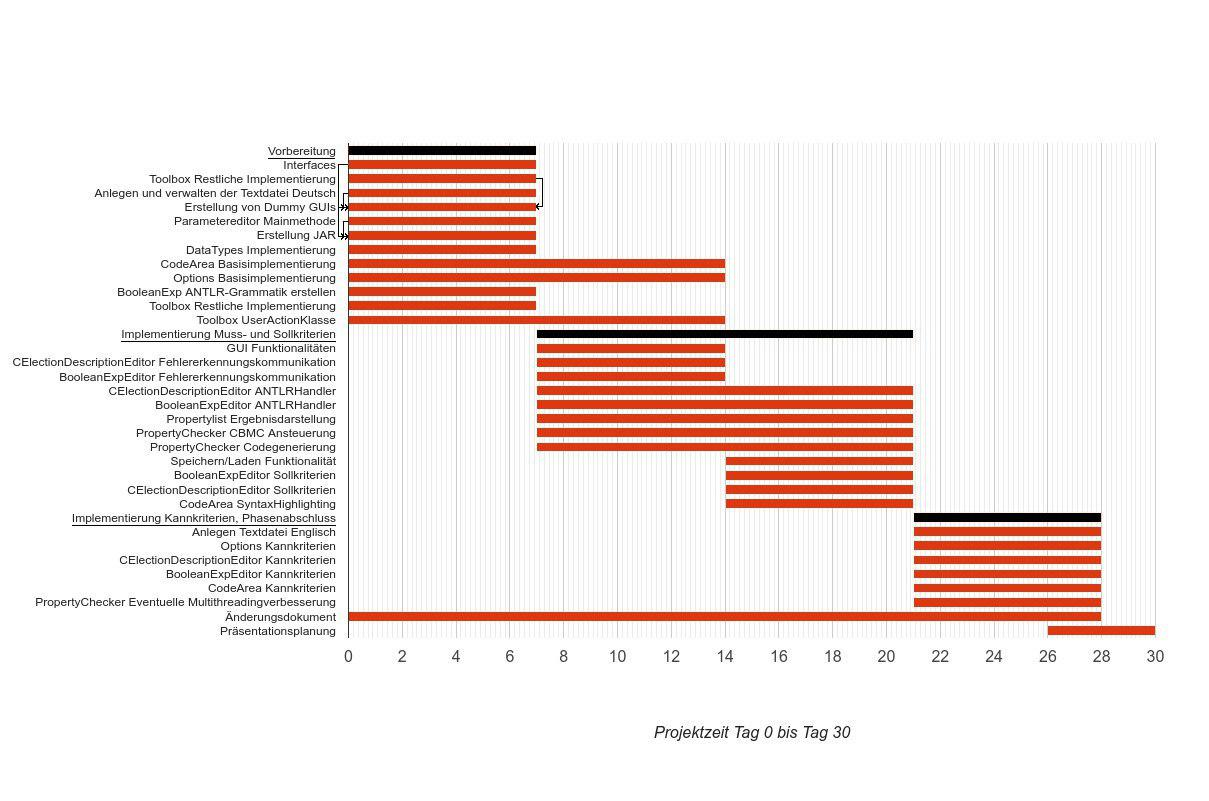
\includegraphics[width=1.3\textwidth] {originalPlanung.jpg}

\section{Eigentlicher Ablauf}
Der ursprüngliche Plan wurde hauptsächlich eingehalten. Ein Paar Komplikationen bei den Paketen \verb!highlevel!, \verb!parametereditor! und \verb!propertylist! verzögerten die Fertigstellung einiger Meilensteine.

(Genauere Beschreibung von Aufgabenumverteilung bzw. Ablaufänderung folgt)

(GANTT Diagramm von tatsächlichem Ablauf folgt)

\end{document}